 \chapter[The 19$^{\text{th}}$ of April 2024 -2D]{2D}

\begin{chapabstract}
	No meeting but notes, ideas and discussions
\end{chapabstract}


\minitoc

\section{Integral formulation of the 2D problem}

\subsection{Training}
\subsubsection{Integral evaluation}
For the integral computation of the loss during the training, no input is required as the only evaluation points for the space quantities are evaluated at the integration points that only depends on the mesh and the order of the elements. 

\Rqs{For the automatic differenciation to be available when computing the loss, the inverse mapping $\mathcal{M}^{-1}$ from the real coordinates to the reference coordinate is used when interpolating the displacement. That allows any derivative to be computed using the automated tools later in the loss. The strain could be directly be derived but that might be a limitation for most complex loss functions.}{The difference between evaluation and training are easily handled by calling the methods
\begin{itemize}
	\item \code{model.train()}
	\item \code{model.eval()}
	\end{itemize}}

\begin{equation}
	\begin{cases}
		\vect{x_g} = \sum\limits_{i = 1}^{N_e} N_i(\vect{\xi_g})\vect{x_i} \\
		\vect{u}\left(\vect{x_g}\right) =  \sum\limits_{i = 1}^{N_e} N_i\left(\underbrace{\mathcal{M}^{-1}\left(\vect{x_g}\right)}_{=\vect{\xi_g}}\right)\vect{u_i } \\[7pt]
		\text{det}\left(J\left(\vect{x_g}\right)\right) = \text{det}\left(\frac{\mathrm{d}\vect{\xi_g}}{\mathrm{d}\vect{x_g}}\right)
	\end{cases}
\end{equation}

\subsubsection{Multi-scale strategy}

In order to speed-up the convergence process the transfer learning capabilities of the HiDeNN framework (described in \cref{chap:Transfer_learning} for the parametric case) are used to spread global information from a coarse scale as an initialisation of a finer scale. Such a training merges the mesh convergence analysis with the computation of a solution at a lower cost, ensuring the quality of the final solution regarding discretisation error. 


The automation of the multi-scale training rely an a convergence criterion of the mesh's size. A first idea is to compute the value of the maximum strain of the last converged mesh and compare it to the value of the previous converged mesh. If stagnation is met then training is stopped otherwise a refinement is performed and the previous coarser solution is used to initialise the finer solution.


\subsubsection{Mesh r-adaptivity}


The iso-stress appears smoother with r-adaptivity as the chequerboard effect is less noticeable as illustrated in \cref{fig:r-adaptivity}

\begin{figure}
	\begin{subfigure}[t]{0.5\linewidth}
		\centering
		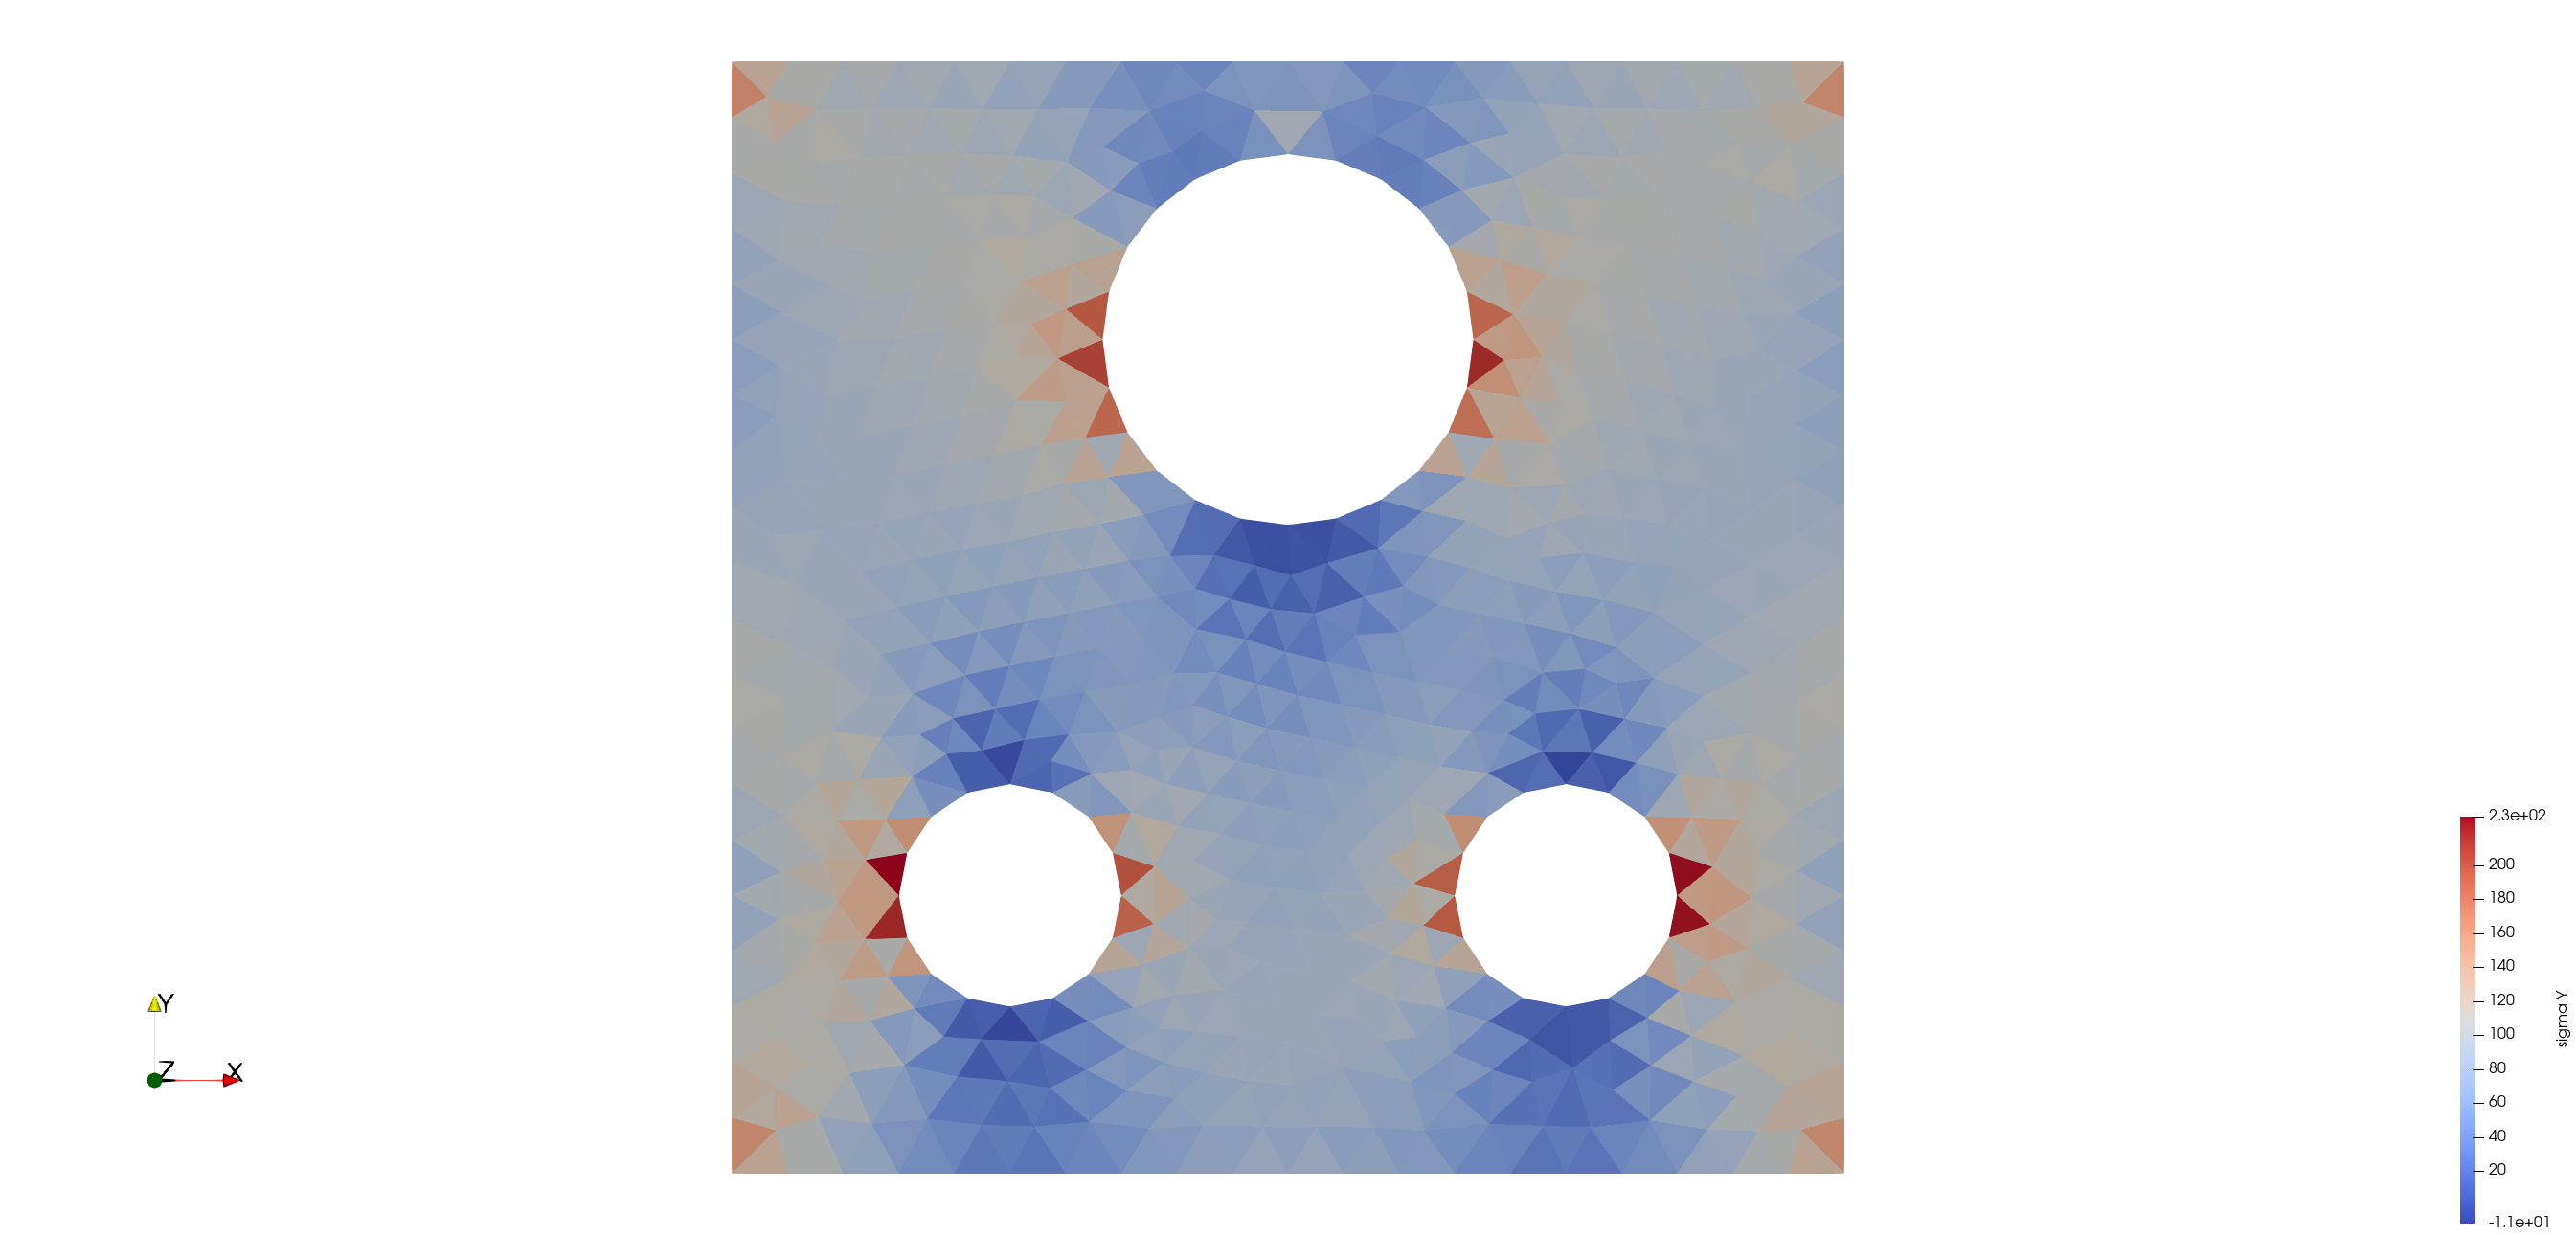
\includegraphics[width=\linewidth]{Figures/Fixed_mesh_sigma_yy.png}
		\caption{$\sigm_{yy}$ stress component on the \\fixed initial mesh}
	\end{subfigure}
	\begin{subfigure}[t]{0.5\linewidth}
		\centering
		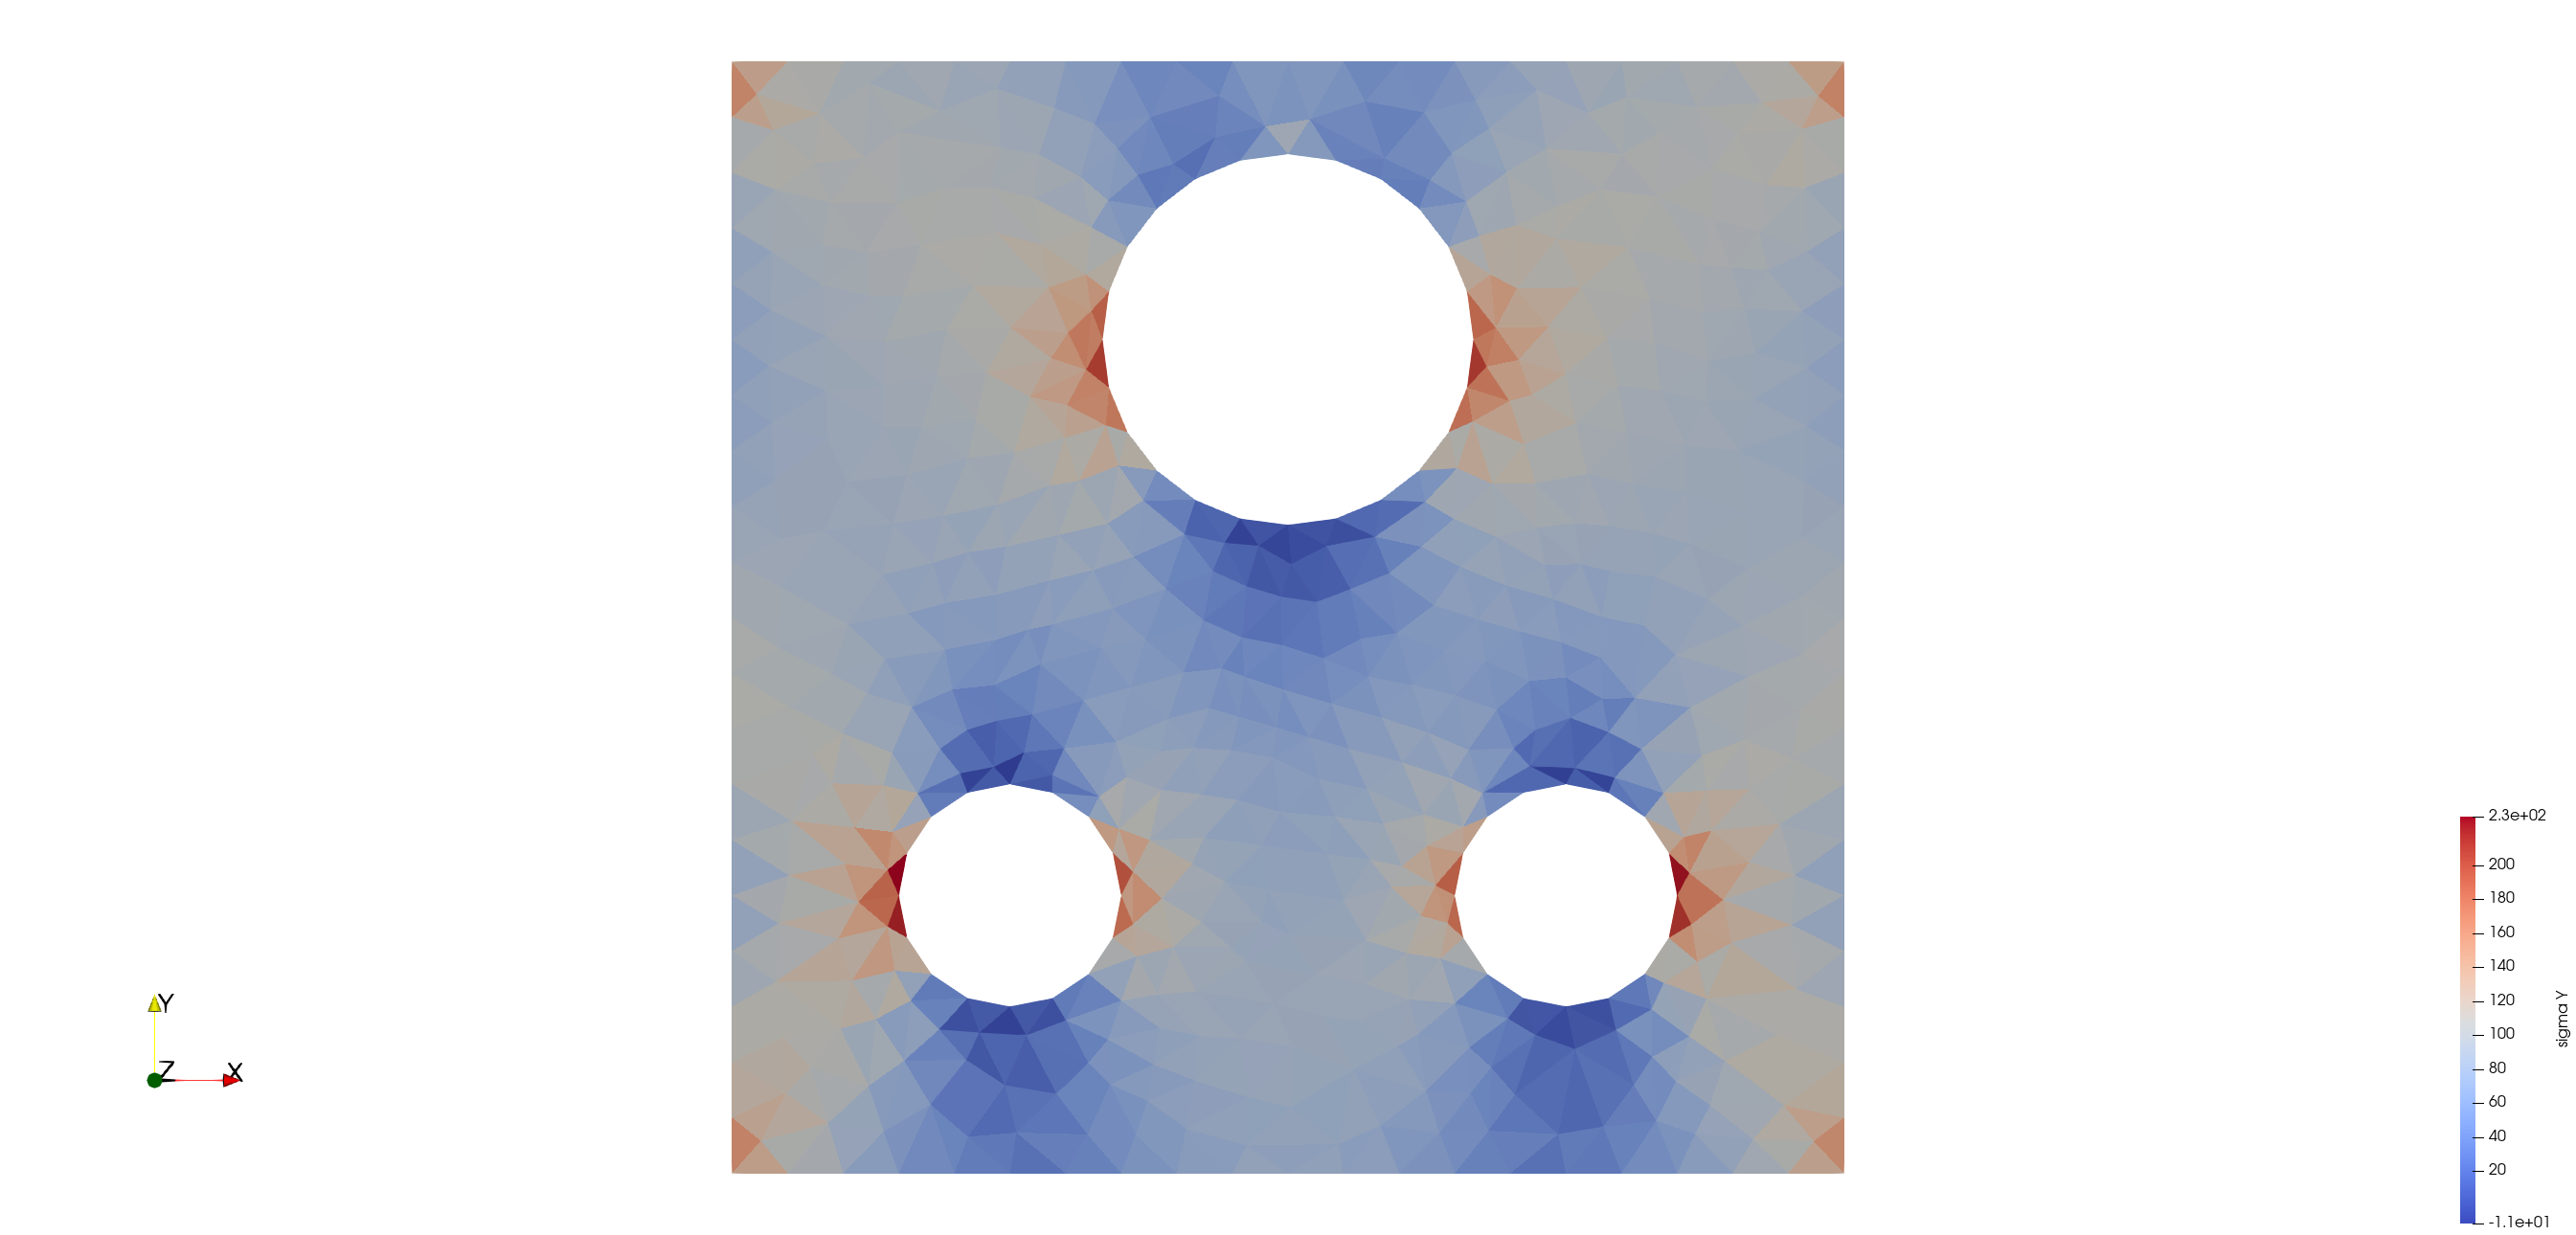
\includegraphics[width=\linewidth]{Figures/Free_mesh_sigma_yy.png}
		\caption{$\sigm_{yy}$ stress component on the \\adapted mesh}
	\end{subfigure}  
	\caption{Influence of mesh adaptivity on the stress}
	\label{fig:r-adaptivity}
\end{figure}


\begin{itemize}
	\item For it to be very efficient we must find a way to do \textit{h-adaptivity}
	\item Instead of uniform refinements, use local refinement (Split T3 elements where the density increased passed a threshold)
	\begin{itemize}
		\item If no recombination, should be fairly easy
	\end{itemize}
\end{itemize}

\subsection{Mesh h-adaptivity}

An idea would be to split the elements whose indexes $I_{ds}$ are

\begin{equation}
	I_{ds} = \argmax_{e}~\frac{\mathrm{d}}{\mathrm{d}t} \left[ \text{det}\left(J\left(x^e_g\right)\right)\right]
\end{equation}

\begin{itemize}
	\item If global refinement needed, set max element size as average current element size on the locally refined mesh.
\end{itemize}


\newpage
\section{Stress admissibility}
The solution is sought after as the pair $\left(\vect{u_{NN}},\sigm_{NN}\right) \in \mathcal{U}  \times \mathcal{S}$, with
\begin{equation}
	\begin{cases}
	\mathcal{U} = \left\{\vect{u} \; | \; \vect{u}\in \mathcal{H}^1\left(\Omega\right)\text{,} 
	\vect{u} = \vect{u}_d \text{ on } \partial \Omega_d \right\}, \\
		\mathcal{S} = \left\{\sigm \; | \; \sigm\in \mathcal{H}\left(\text{div}\right)\text{,} 
	\sigm\vect{n} = \vect{F}_d \text{ on } \partial \Omega_N \right\}, 
	\end{cases}
\end{equation}
by minimising a cost function 
\begin{equation}
	\mathcal{L} = \underbrace{\Vert \text{\textbf{div}}\left(\sigm_{NN}\right)+\vect{f}\Vert}_{\mathcal{L}_{\text{PDE}}} + \underbrace{ \Vert \sigm_{NN} - \ftensor{K}:\eps\left(\vect{u_{NN}}\right) \Vert_{2}}_{\mathcal{L}_{\text{const}}}
\end{equation} consisting of a constitutive error term $\mathcal{L}_{\text{const}}$ and a PDE residual term $\mathcal{L}_{\text{PDE}}$.
\subsection{Constitutive error}
\paragraph{Definition}
In the mixed formulation, the interpolated stress $\sigm_{NN} \in \mathcal{H}\left(\text{div}\right)$ is divergence free while the displacement-derived stress $\sigm\left(\vect{u_{NN}}\right) \notin \mathcal{H}\left(\text{div}\right)$ is not as $\vect{u_{NN}}\in \mathcal{H}^1\left(\Omega\right)$ only. Static admissibility can only be weakly satisfied and the strong form of the equilibrium is not satisfied by the displacement field. The constitutive error
\begin{equation}
	\Psi\left(\vect{u_{NN}},\sigm_{NN}\right) = \frac{1}{2} \Vert \sigm_{NN} - \ftensor{K}:\eps\left(\vect{u_{NN}}\right) \Vert_{\ftensor{K}} \neq \frac{1}{2} \mathcal{L}_{\text{const}}
	\label{eq:EC}
\end{equation}
not being zero at convergence illustrates that idea. 
\Rq{If the constitutive term in the loss is computed using a MSE, it differs from the CRE computed with the energetic norm. In a tchnical aspect a difference lies in the fact that the size of the element is accounted for in via the jacobian of the elements in the intergal form while the sum of the MSE depends strongly on the sampling points where the error is estimated.}

\paragraph{Decoupling of the two fields}

\begin{equation}
	\begin{split}
			2~\Psi\left(\vect{u},\sigm\right) & =  \intV \left(\sigm - \ftensor{K}:\eps\left(\vect{u}\right)\right) : \ftensor{K}^-{-1}:\left(\sigm - \ftensor{K}:\eps\left(\vect{u}\right)\right) \dV\\ 
			& = \underbrace{\intV \sigm: \ftensor{K}^{-1}: \sigm \dV}_{2U\left(\sigm\right)} + \underbrace{\intV \eps\left(\vect{u}\right):\ftensor{K}:\eps\left(\vect{u}\right) \dV}_{2U\left(\vect{u}\right)}+ 2\intV\sigm:\eps\left(\vect{u}\right)\dV\\
			& = 2~ U\left(\sigm\right) +2~ U\left(\vect{u}\right) - 2\intV\sigm:\eps\left(\vect{u}\right)\dV.\\
	\end{split}
\end{equation}
If we then inject the equilibrium 
\begin{equation}
	\intV\sigm:\eps\left(\vect{u}\right)~\dV = \intS \left(\sigm\vect{n}\right) \cdot \vect{u_d}~\dS +  \intS \vect{F_d}\cdot \vect{u} ~\dS +\intV \vect{f_v}\cdot\vect{u}~\dV,
\end{equation}
in the previous results the constitutive error reads 
\begin{equation}
		\begin{split}
			\Psi\left(\vect{u},\sigm\right)  & = \underbrace{U\left(\sigm\right) - \intSd \left(\sigm\vect{n}\right) \cdot \vect{u_d}~\dS }_{E_p\left(\sigm\right)} +\underbrace{U\left(\vect{u}\right) -  \intSn \vect{F_d}\cdot \vect{u} ~\dS -\intV \vect{f_v}\cdot\vect{u}~\dV}_{E_p\left(\vect{u}\right)}\\
			& =E_p\left(\sigm\right)+E_p\left(\vect{u}\right).
		\end{split}
\end{equation}
\Rq{We would then get a constitutive error that accounts for both the CRE and the equilibrium, thus there would be no need for the PDE term in the loss.}
Therefore, minimising the constitutive error consists in finding 

\begin{equation}
	\left(\vect{u_{NN}},\sigm_{NN}\right) = \argmin_{\vect{u}\in \mathcal{U}, \sigm \in \mathcal{S}} \left(\Psi\left(\vect{u},\sigm\right)\right) =  \left(\argmin_{\vect{u}\in \mathcal{U}}E_p\left(\vect{u}\right),\argmin_{\sigm\in \mathcal{S}}E_p\left(\sigm\right)\right),
\end{equation}
But this statement does not hold with the $\mathcal{L}^2$-norm used in the actual loss or without using the equilibrium.